\chapter[Tau leptons][Tau leptons]{Tau leptons}
\label{chap:taus}

\begin{quote}
  Tau leptons and their signature in the ATLAS detector are described. 
\end{quote}

\section{Tau leptons}
\label{sec:taus-theory}

\begin{figure}[tp]
  \centering
  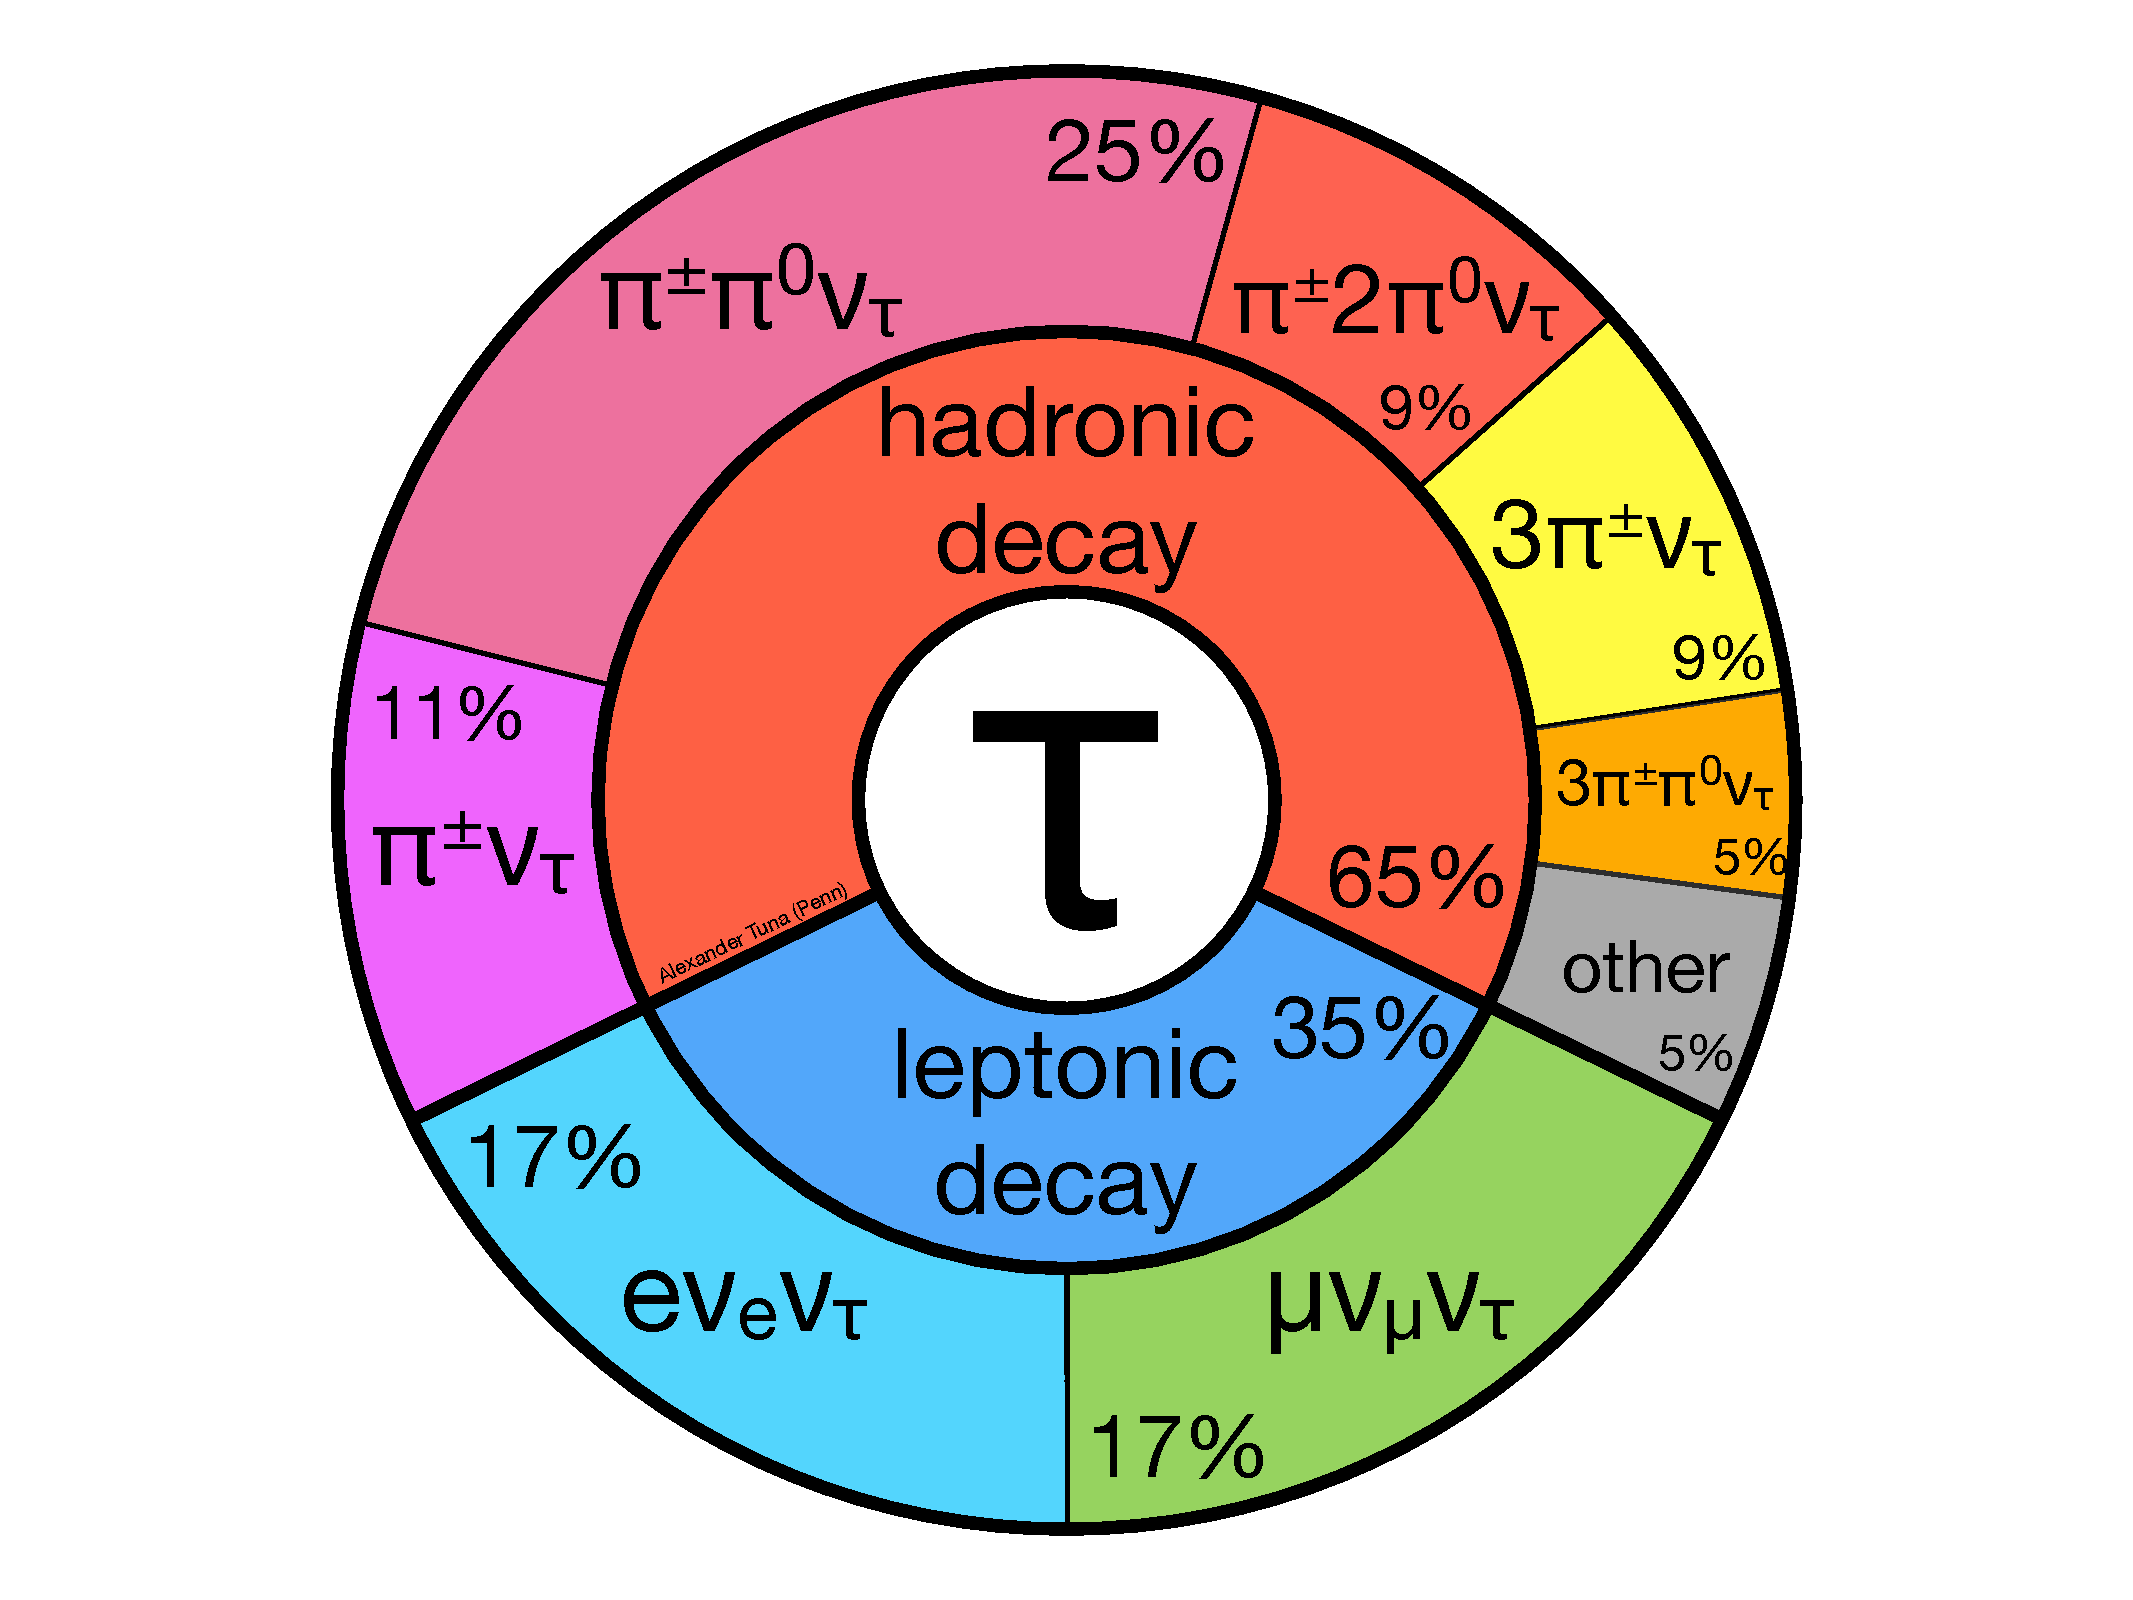
\includegraphics[width=0.48\textwidth]{figures/piecharts/taudecay}
  \caption{Variables.}
  \label{fig:taus-decaypie}
\end{figure}

\section{Leptonic tau decays, $\taul$}
\label{sec:taus-leptons}

\begin{figure}[tp]
  \centering
  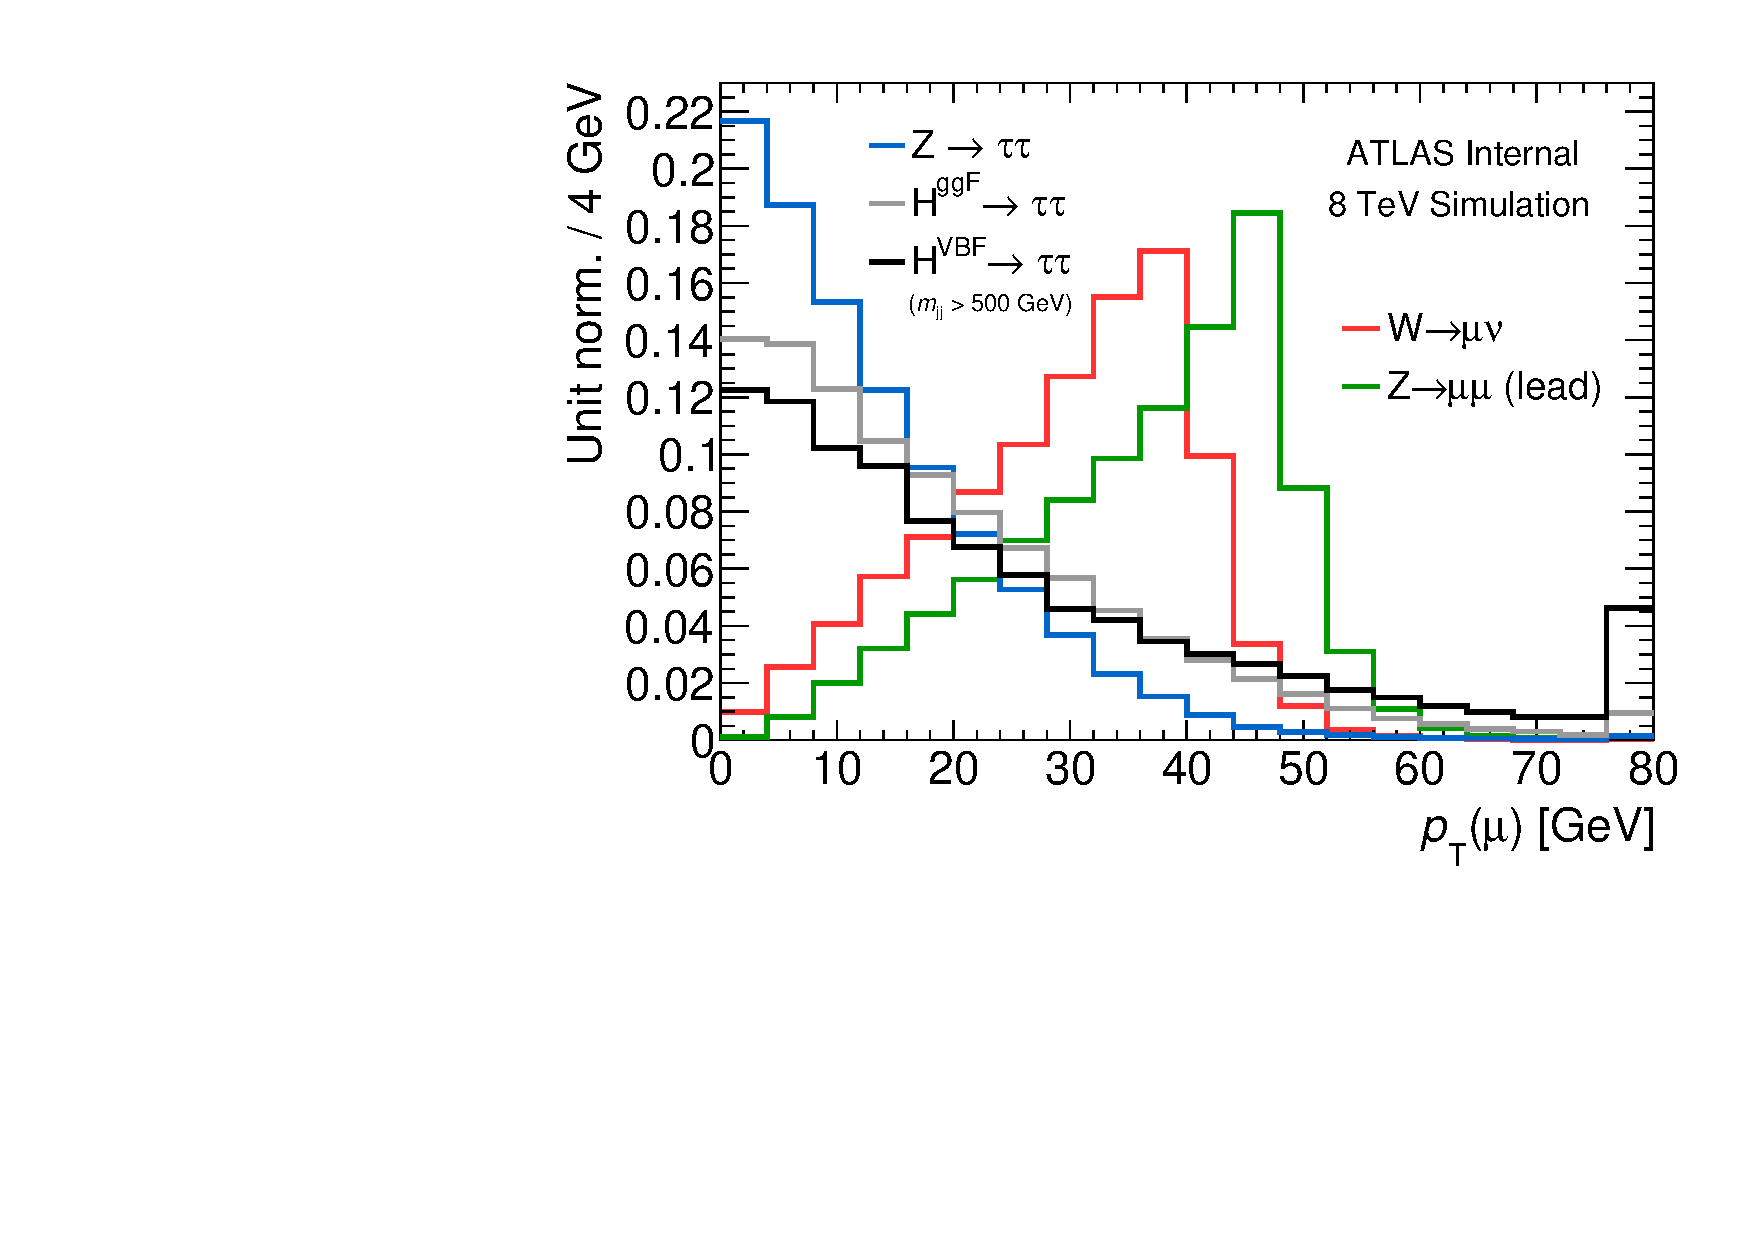
\includegraphics[width=0.7\textwidth]{figures/tauperformance/leptonsfromtausaresoft}
  \caption{Variables.}
  \label{fig:taus-leptonpt}
\end{figure}

\section{Hadronic tau decays, $\tauh$}
\label{sec:taus-jetfakes}

This is a citation~\cite{2014.PERF-2013-06}. Here is a citation~\cite{1999.ATLAS.Physics-TDR}.

\begin{figure}[tp]
  \centering
  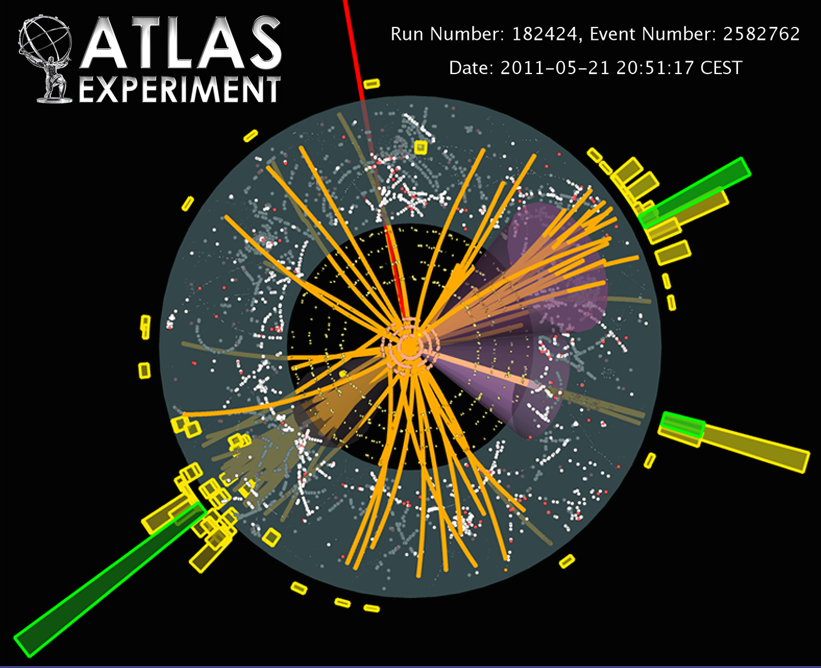
\includegraphics[width=0.95\textwidth]{figures/tauperformance/vp1_3dcocktail_run182424_evt2582762_tttaumu}
  \caption{Variables.}
  \label{fig:taus-eventdisplay}
\end{figure}

\begin{figure}[tp]
  \centering
  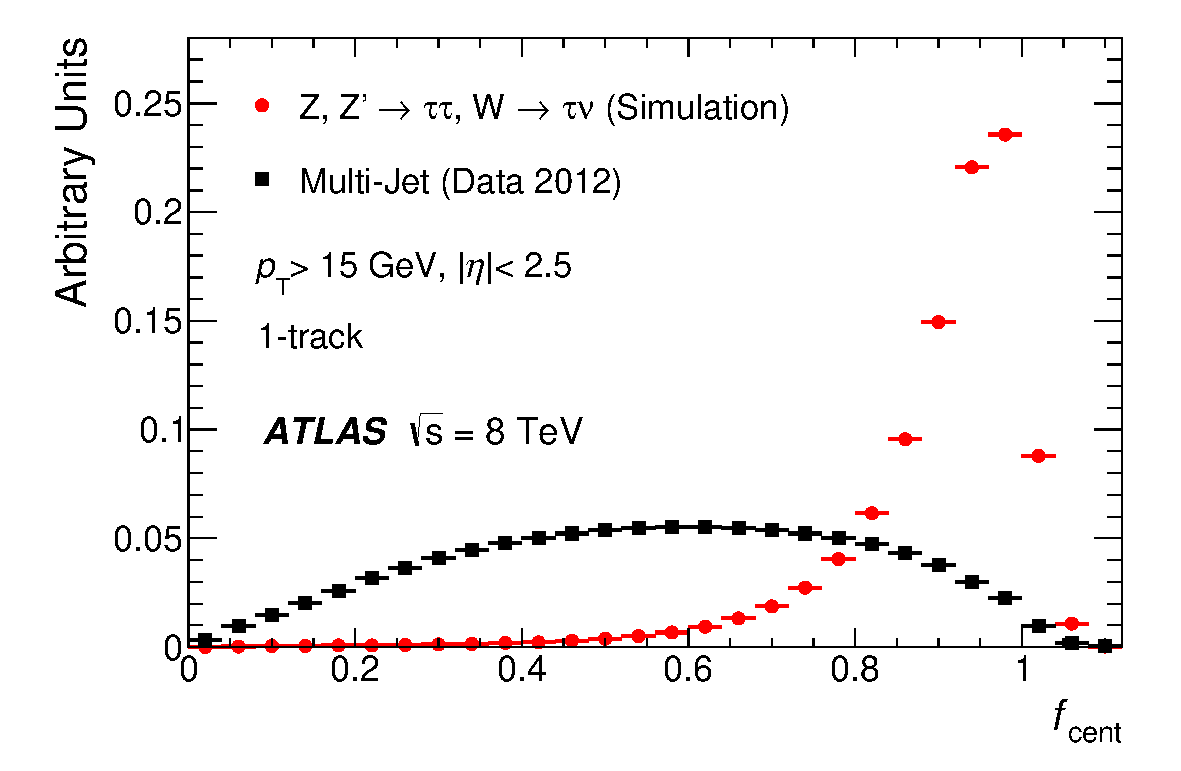
\includegraphics[width=0.48\textwidth]{figures/PERF-2013-06/fig_02a}
  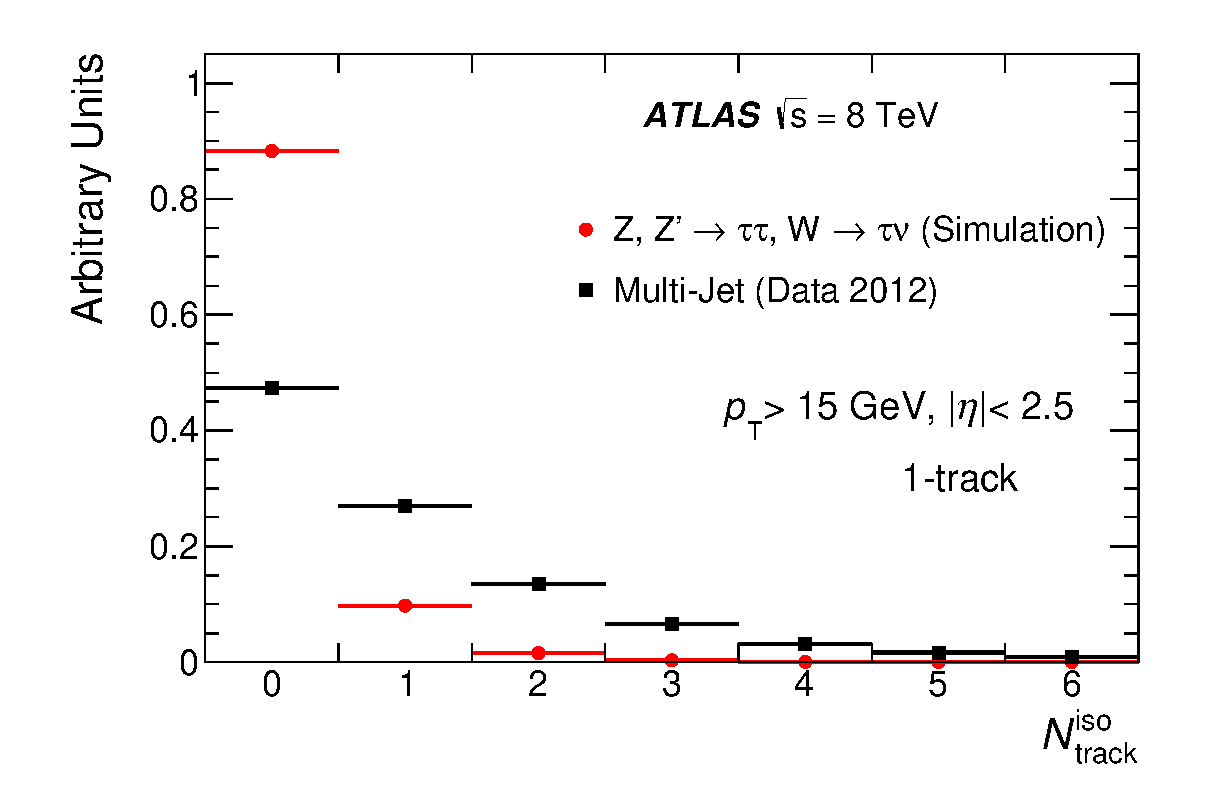
\includegraphics[width=0.48\textwidth]{figures/PERF-2013-06/fig_02b}
  \caption{Variables.}
  \label{fig:taus-id1p}
\end{figure}

\begin{figure}[tp]
  \centering
  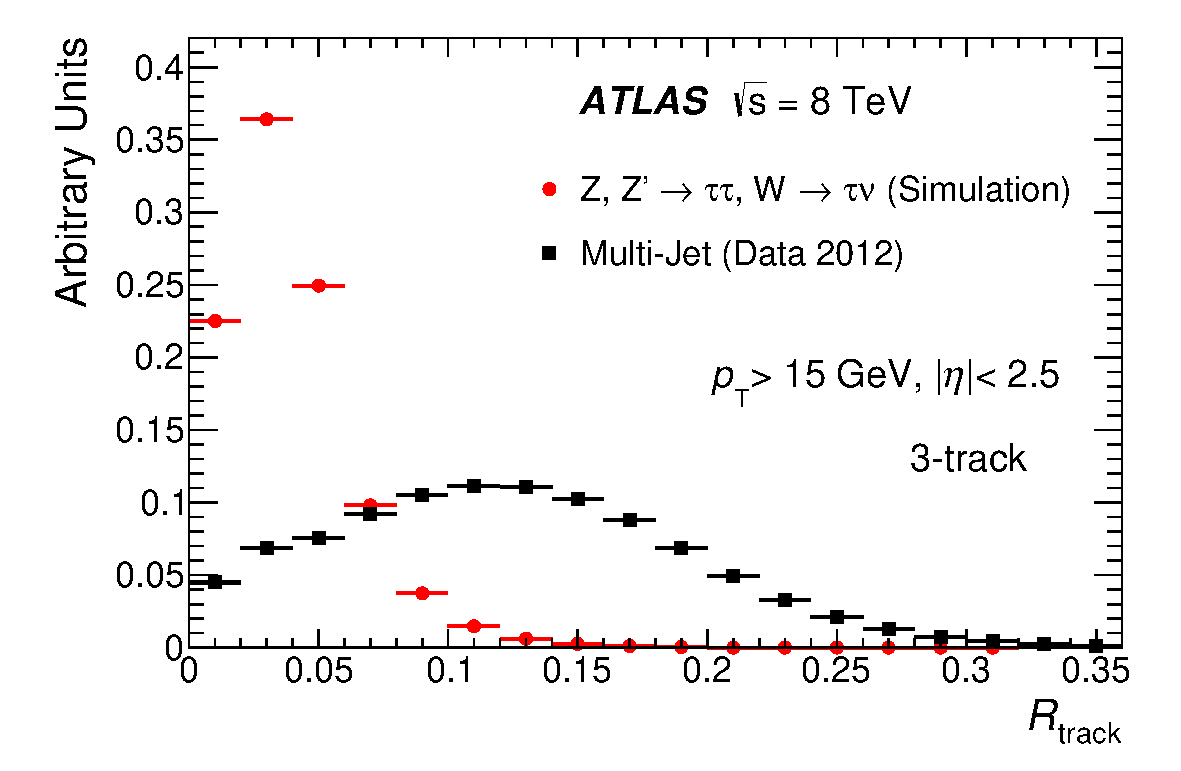
\includegraphics[width=0.48\textwidth]{figures/PERF-2013-06/fig_03a}
  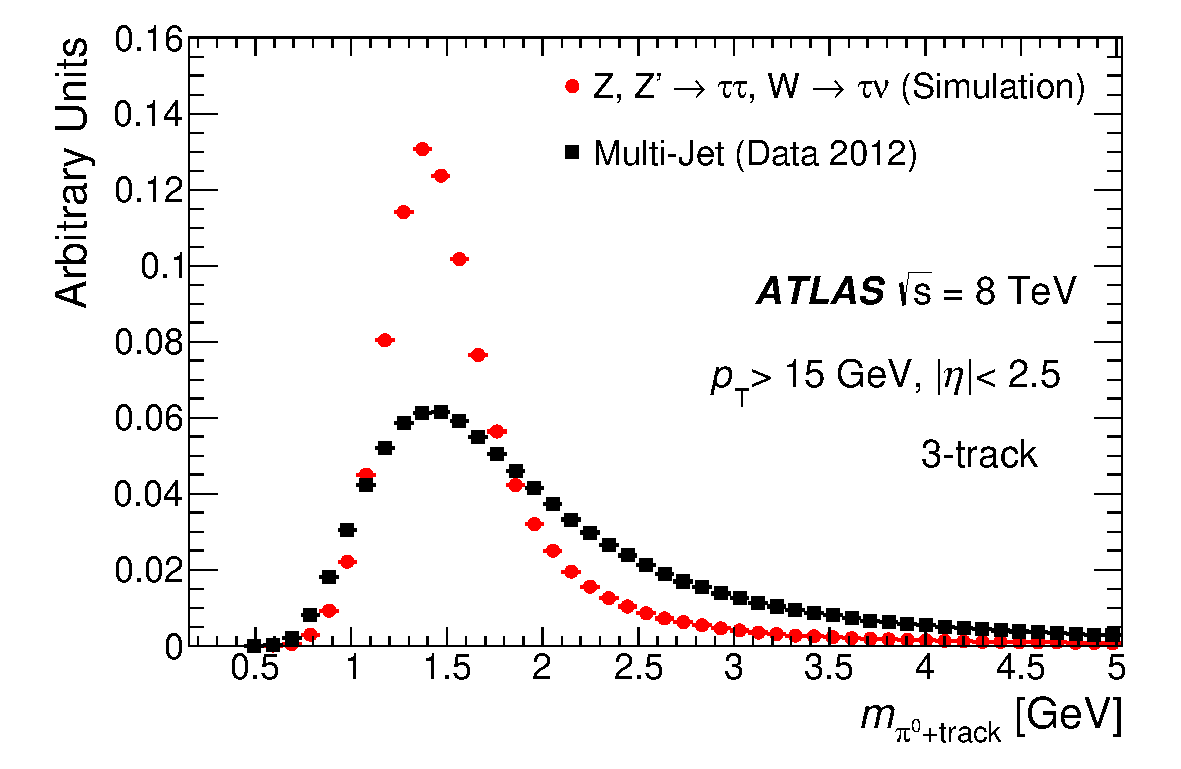
\includegraphics[width=0.48\textwidth]{figures/PERF-2013-06/fig_03b}
  \caption{Variables.}
  \label{fig:taus-id3p}
\end{figure}

\begin{figure}[tp]
  \centering
  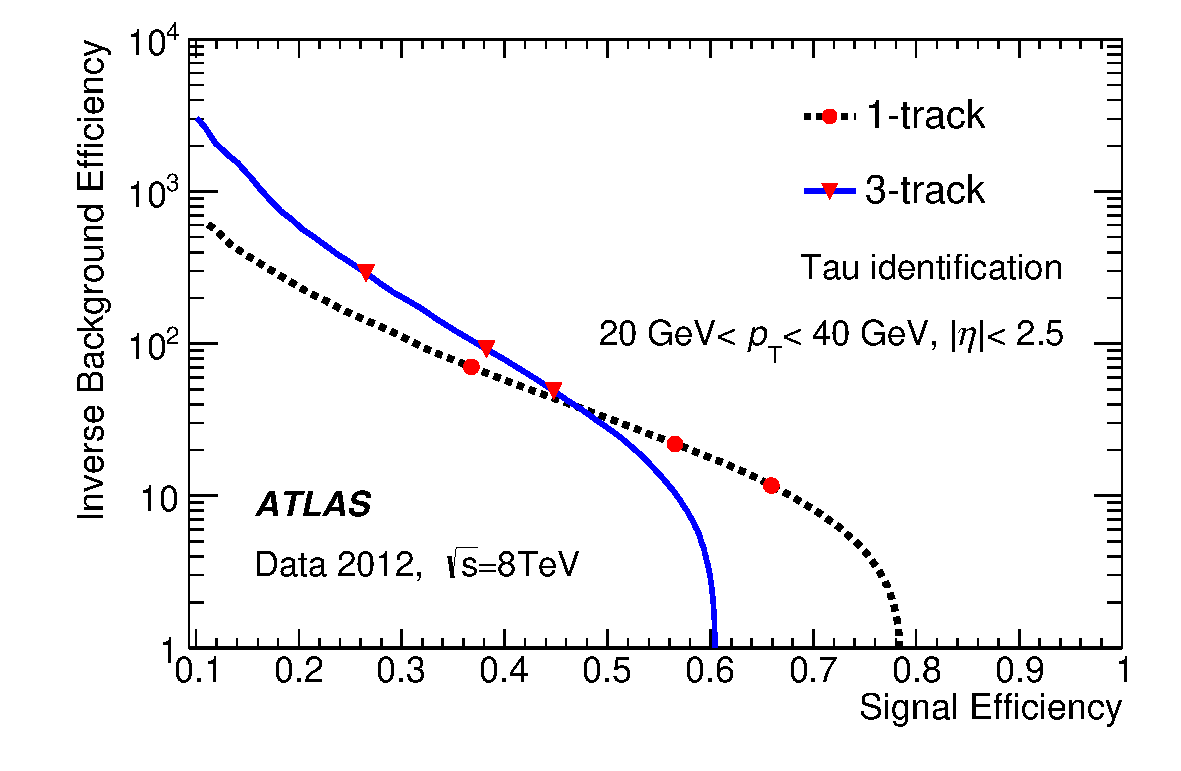
\includegraphics[width=0.48\textwidth]{figures/PERF-2013-06/fig_05a}
  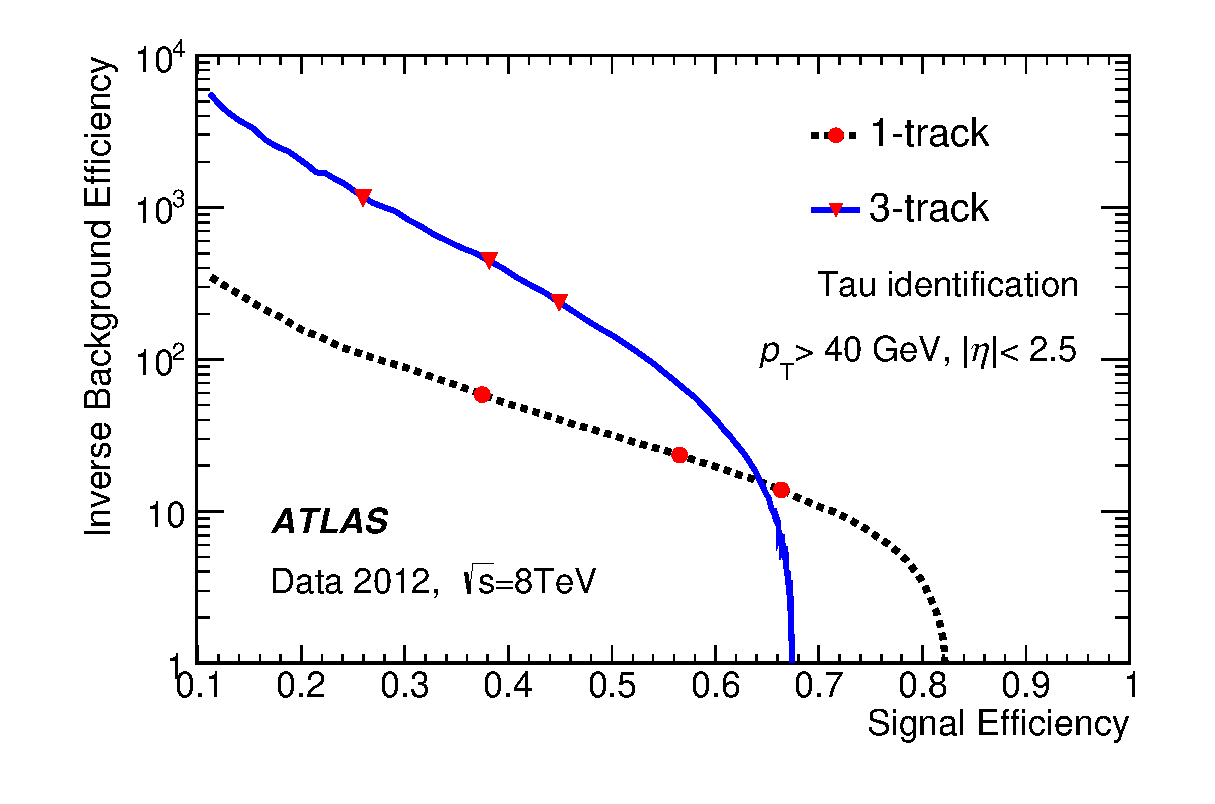
\includegraphics[width=0.48\textwidth]{figures/PERF-2013-06/fig_05b}
  \caption{Variables.}
  \label{fig:taus-idroc}
\end{figure}

\section{Leptons mis-identified as $\tauh$}
\label{sec:taus-leptonfakes}

\begin{figure}[tp]
  \centering
  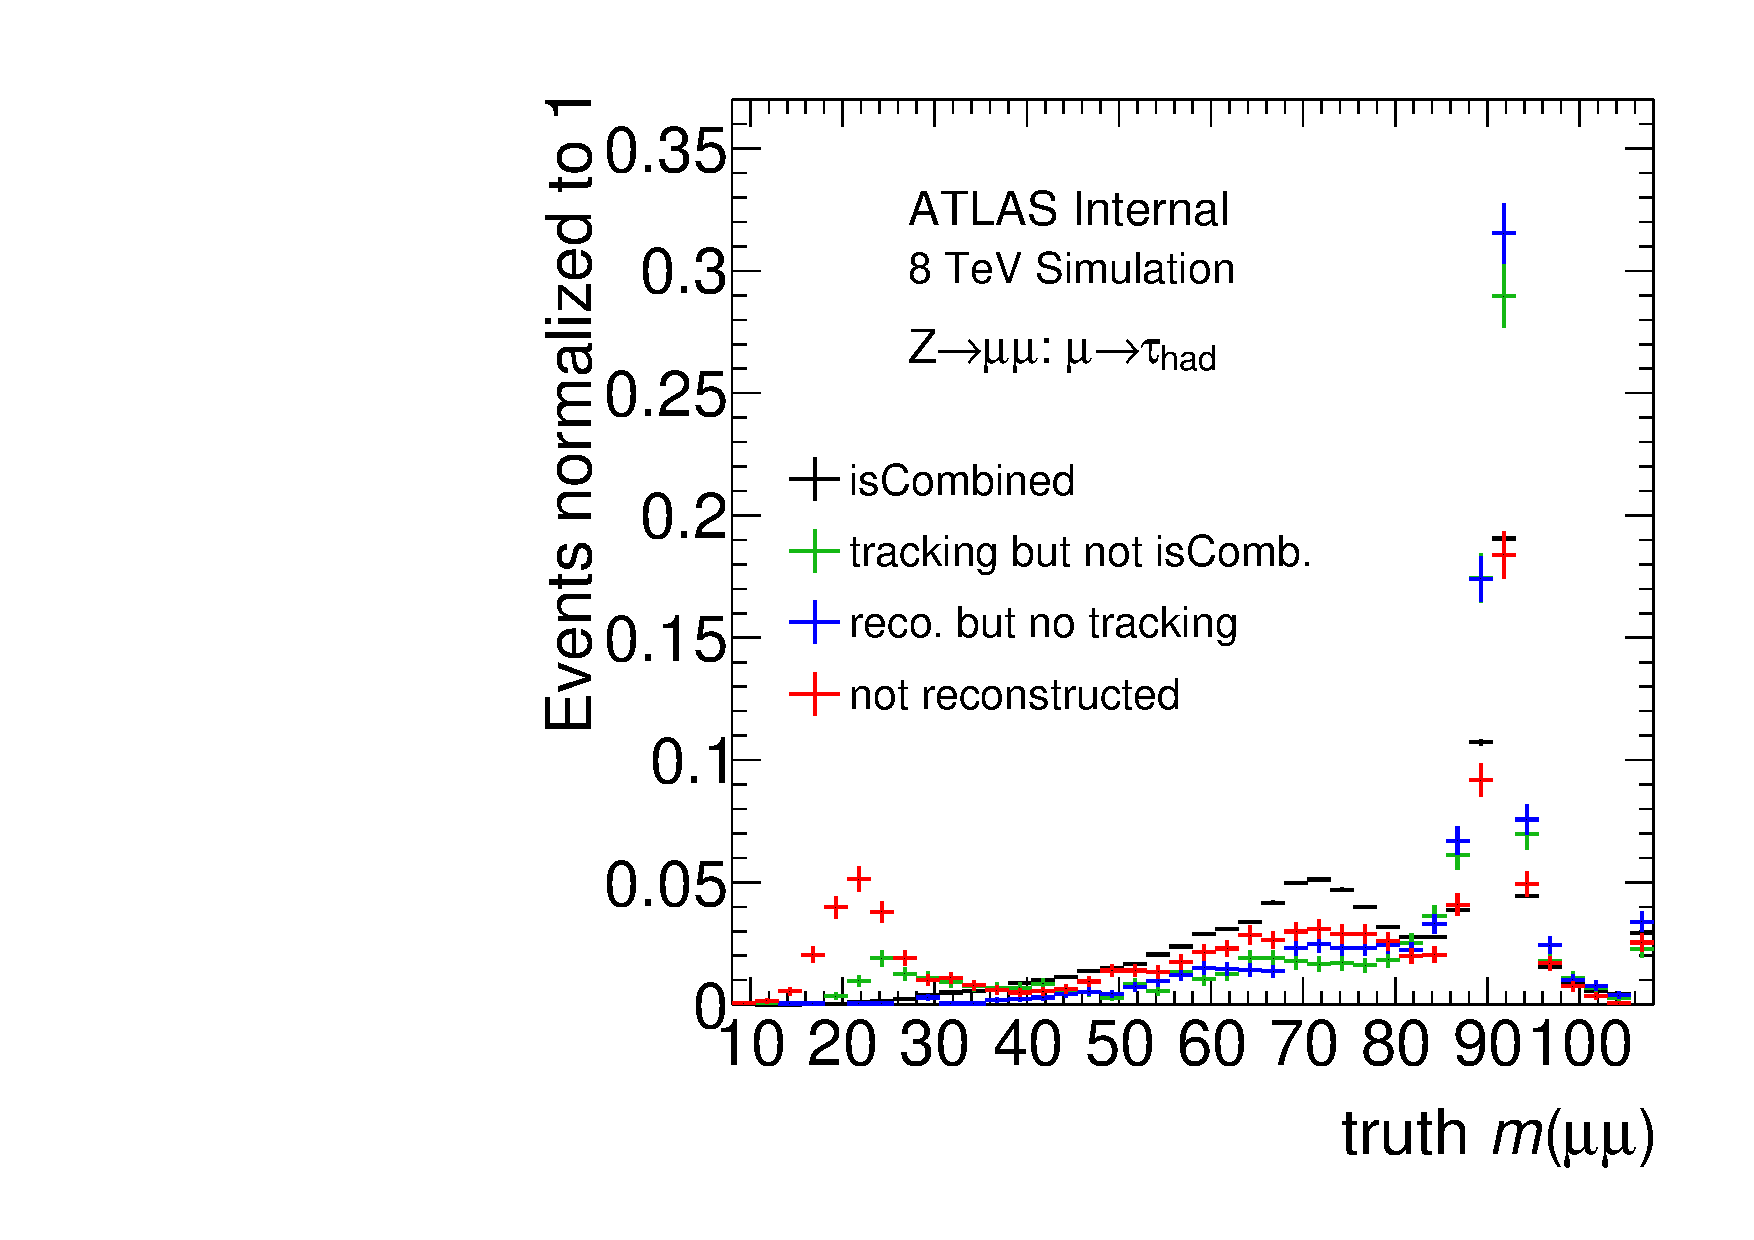
\includegraphics[width=0.48\textwidth]{figures/tauperformance/muonfakes_mll}
  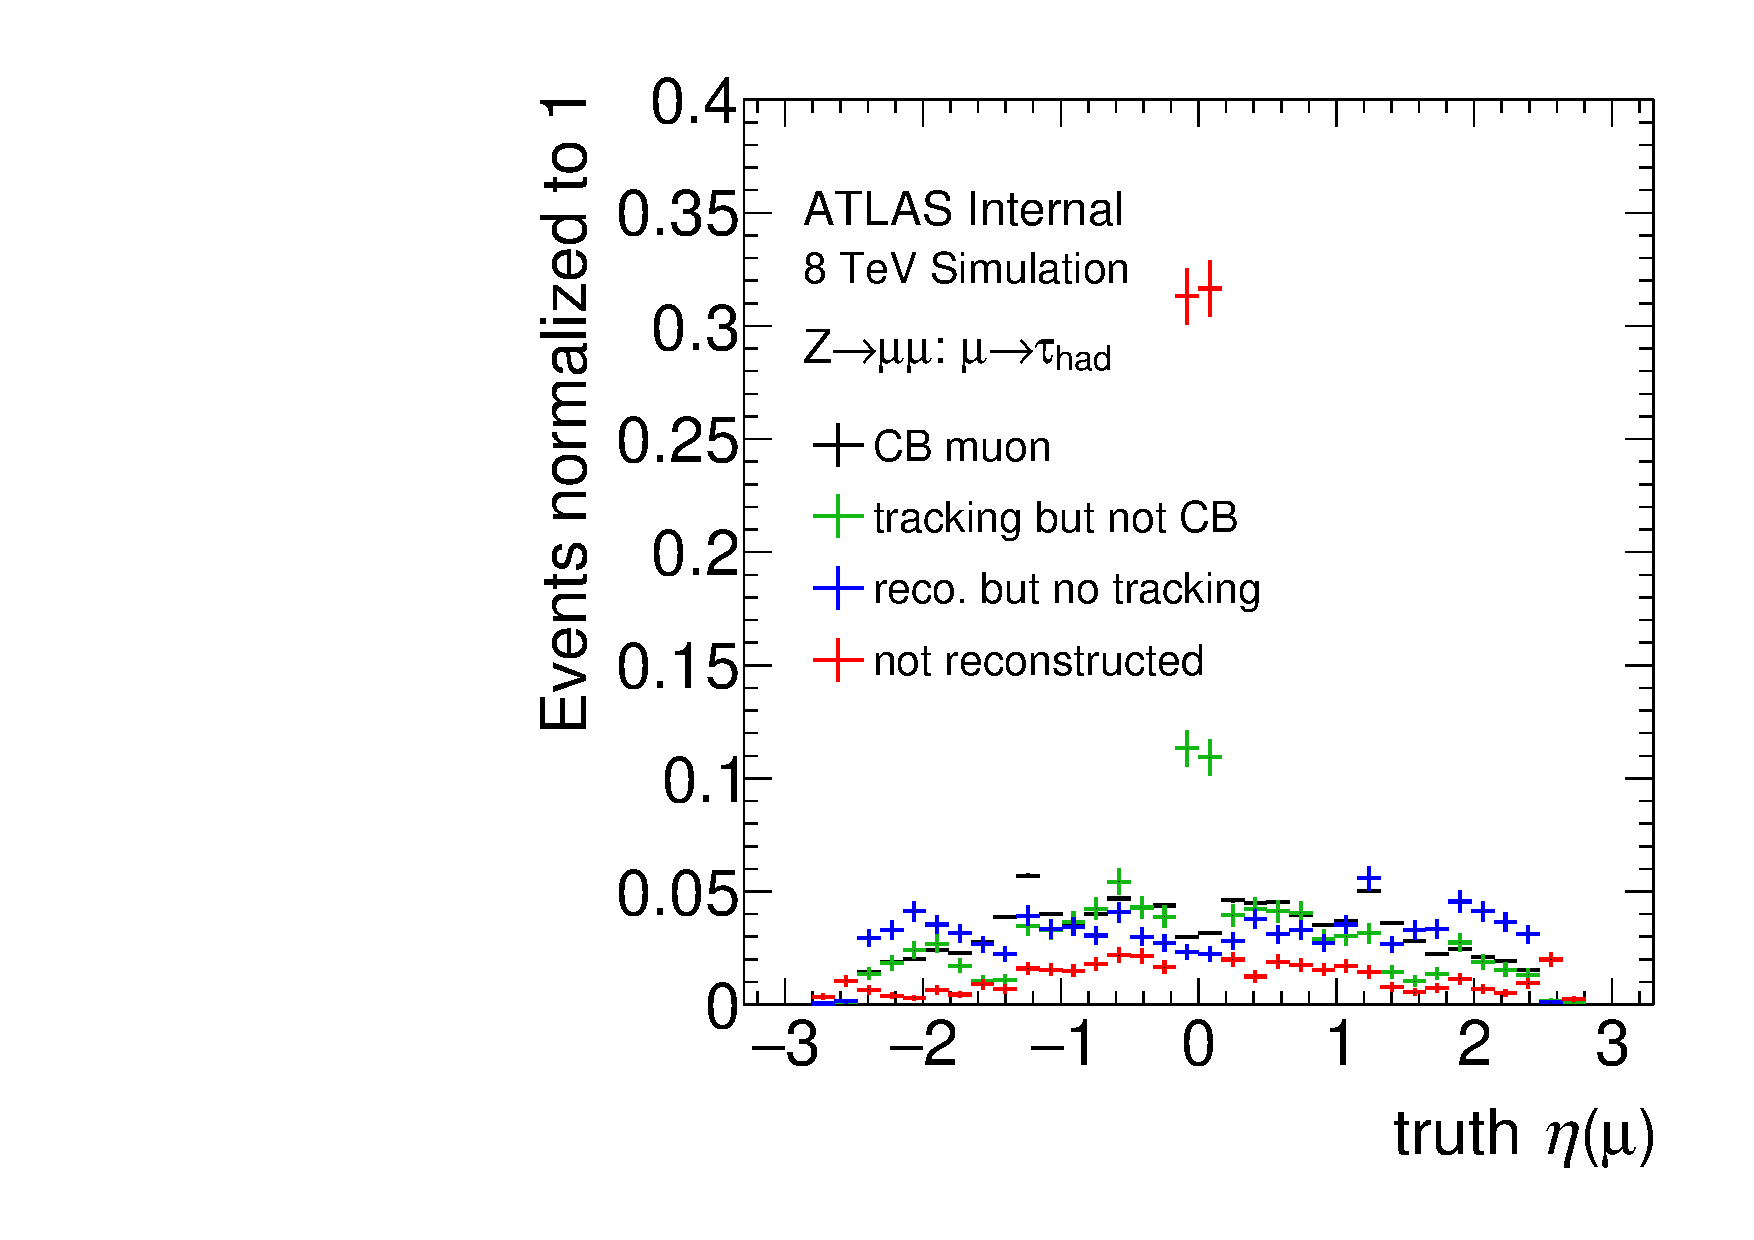
\includegraphics[width=0.48\textwidth]{figures/tauperformance/muonfakes_eta}
  \caption{Variables.}
  \label{fig:taus-muonfakes1}
\end{figure}

\begin{figure}[tp]
  \centering
  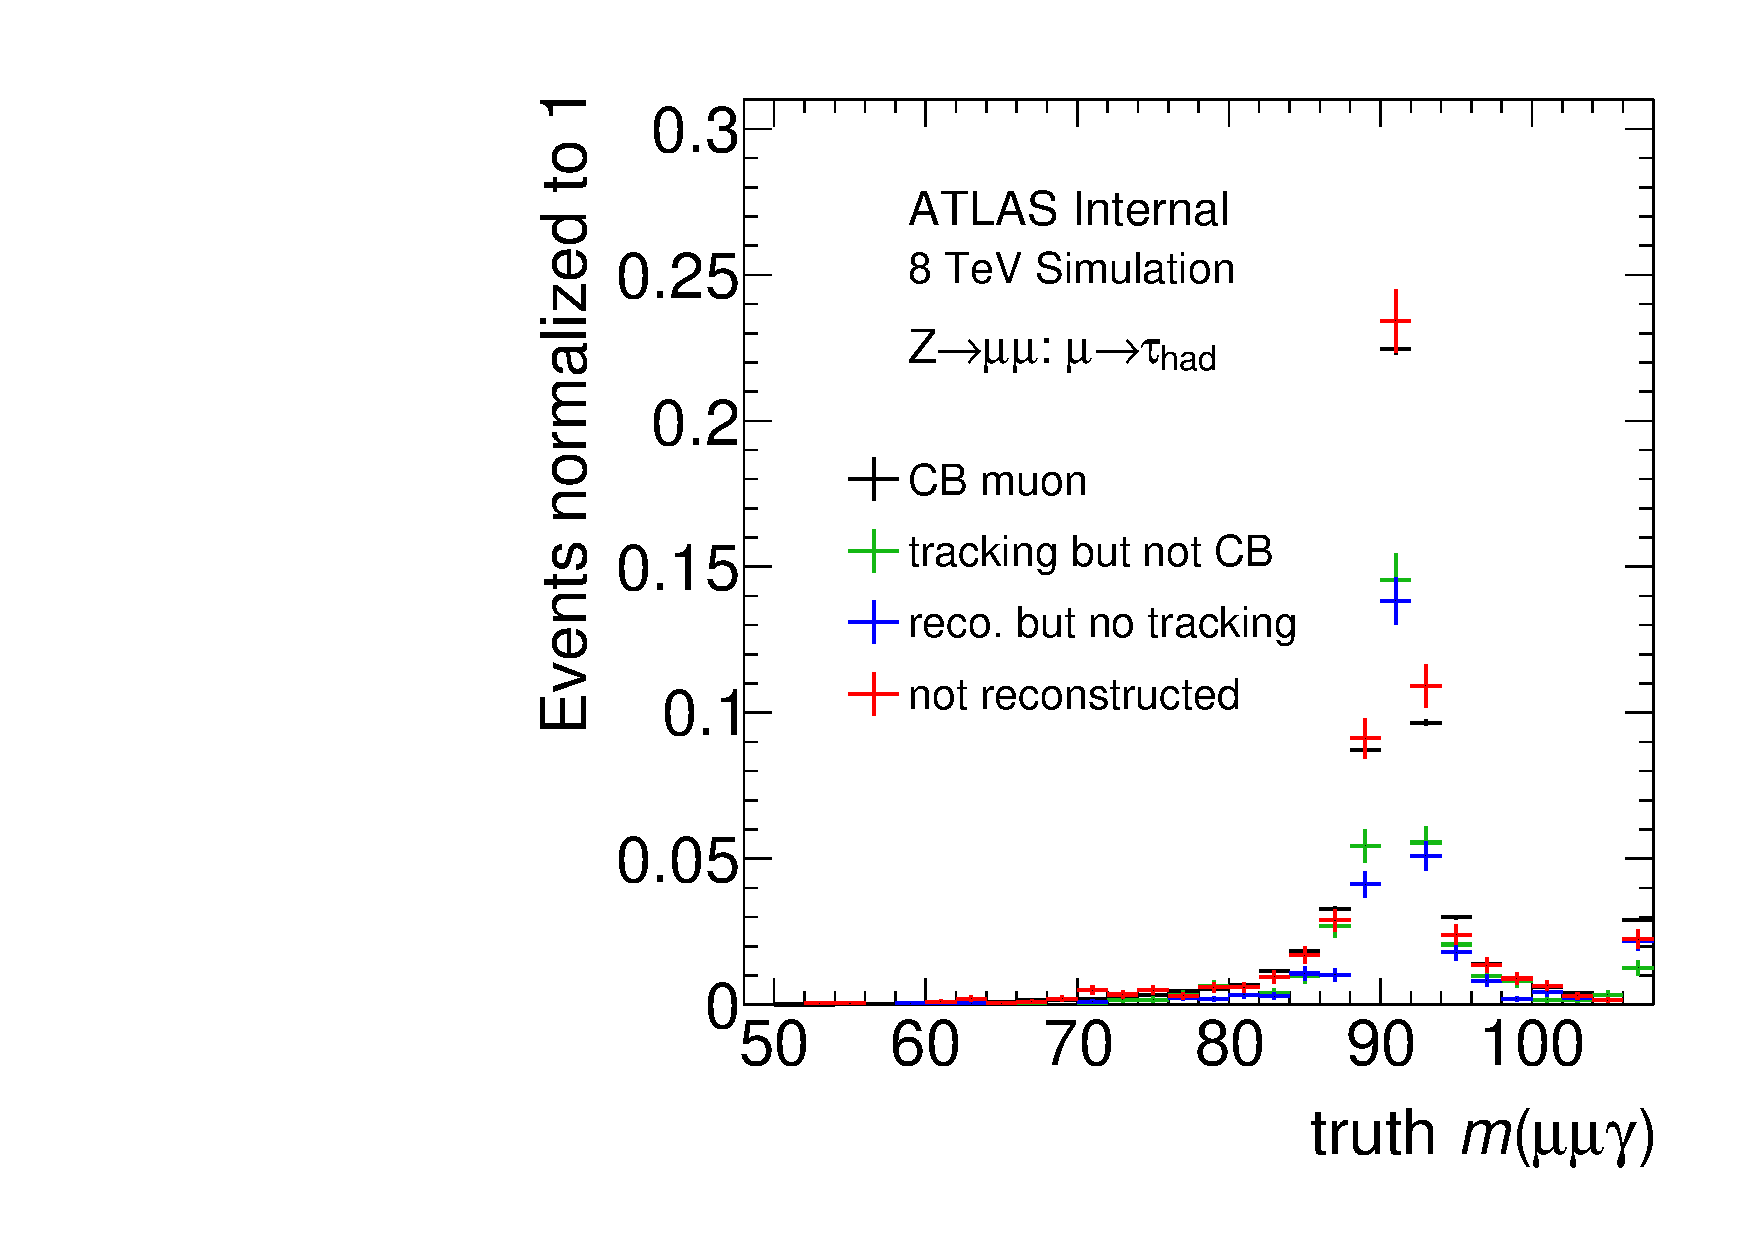
\includegraphics[width=0.48\textwidth]{figures/tauperformance/muonfakes_mlly}
  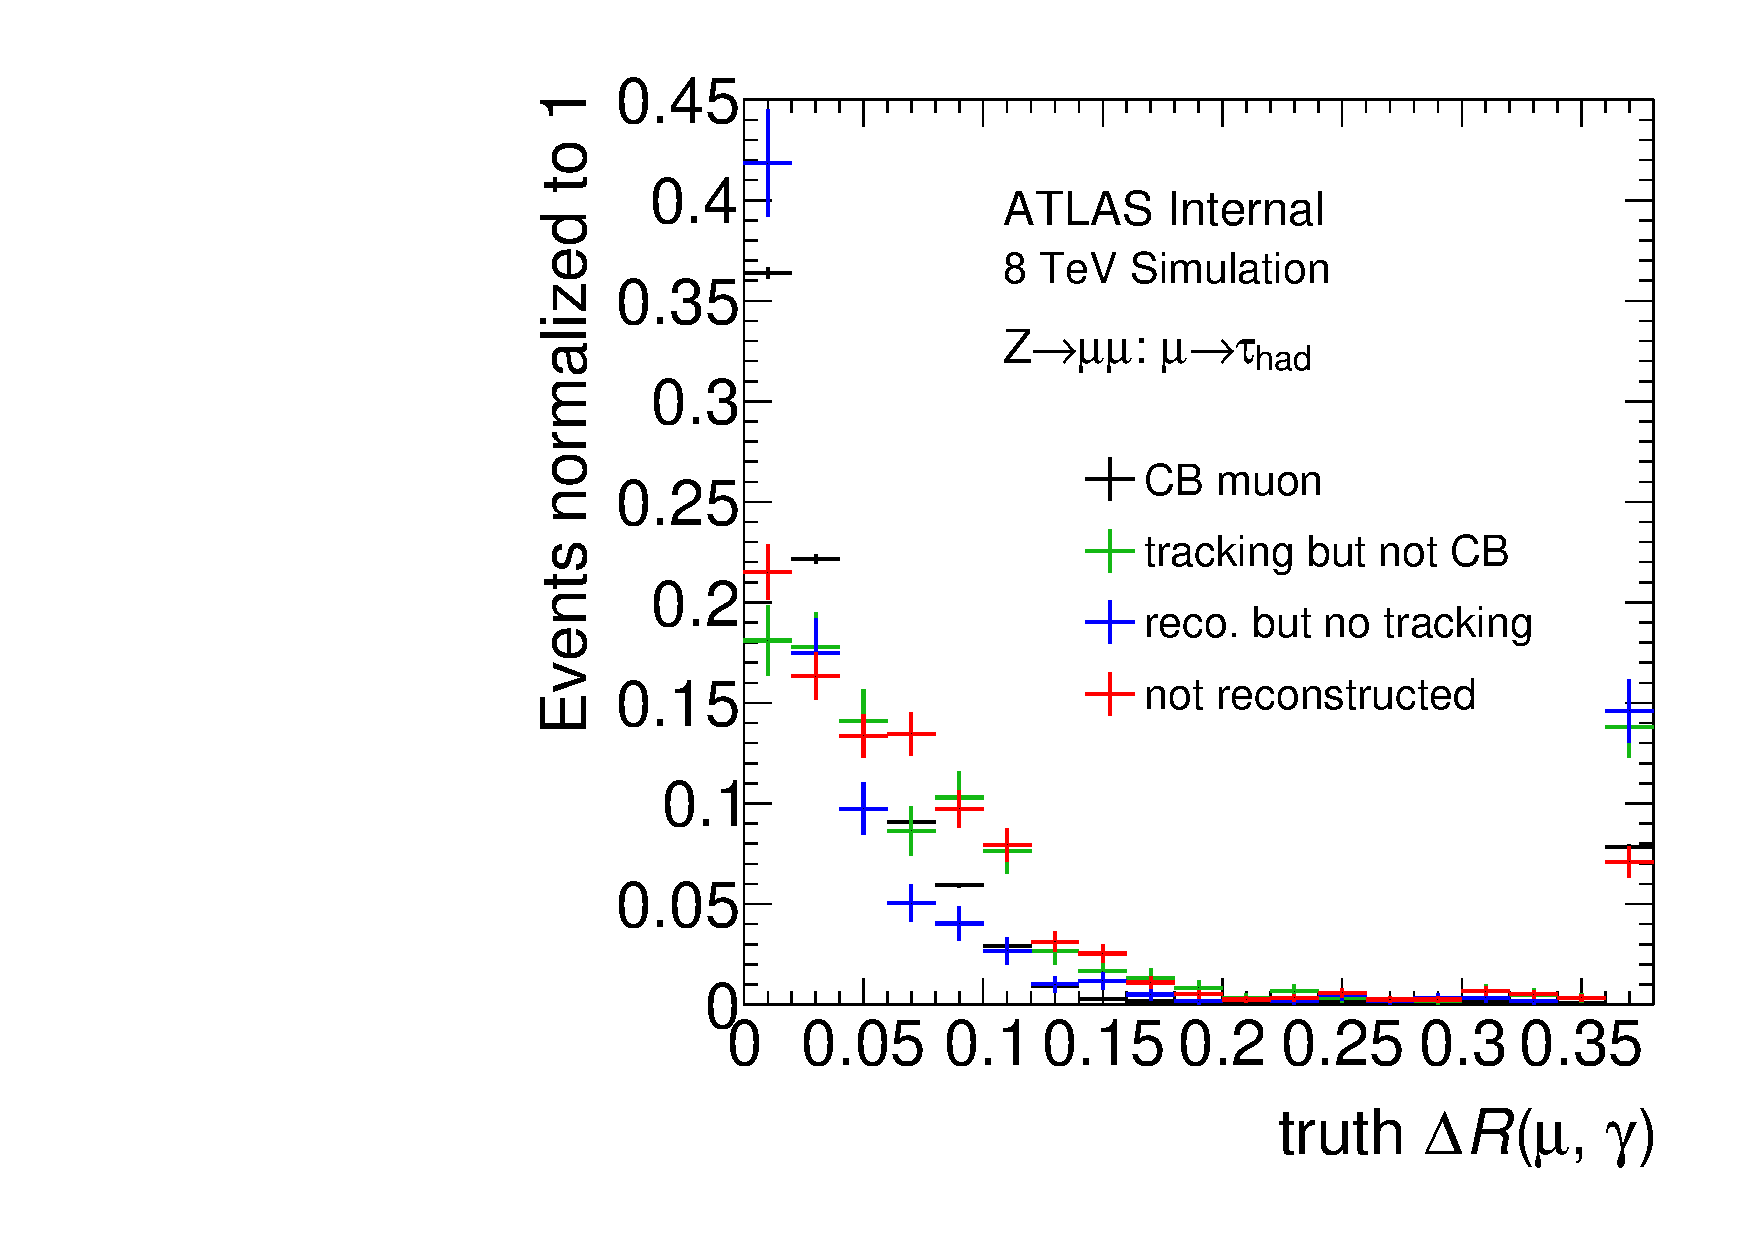
\includegraphics[width=0.48\textwidth]{figures/tauperformance/muonfakes_dR}
  \caption{Variables.}
  \label{fig:taus-muonfakes2}
\end{figure}

\begin{figure}[tp]
  \centering
  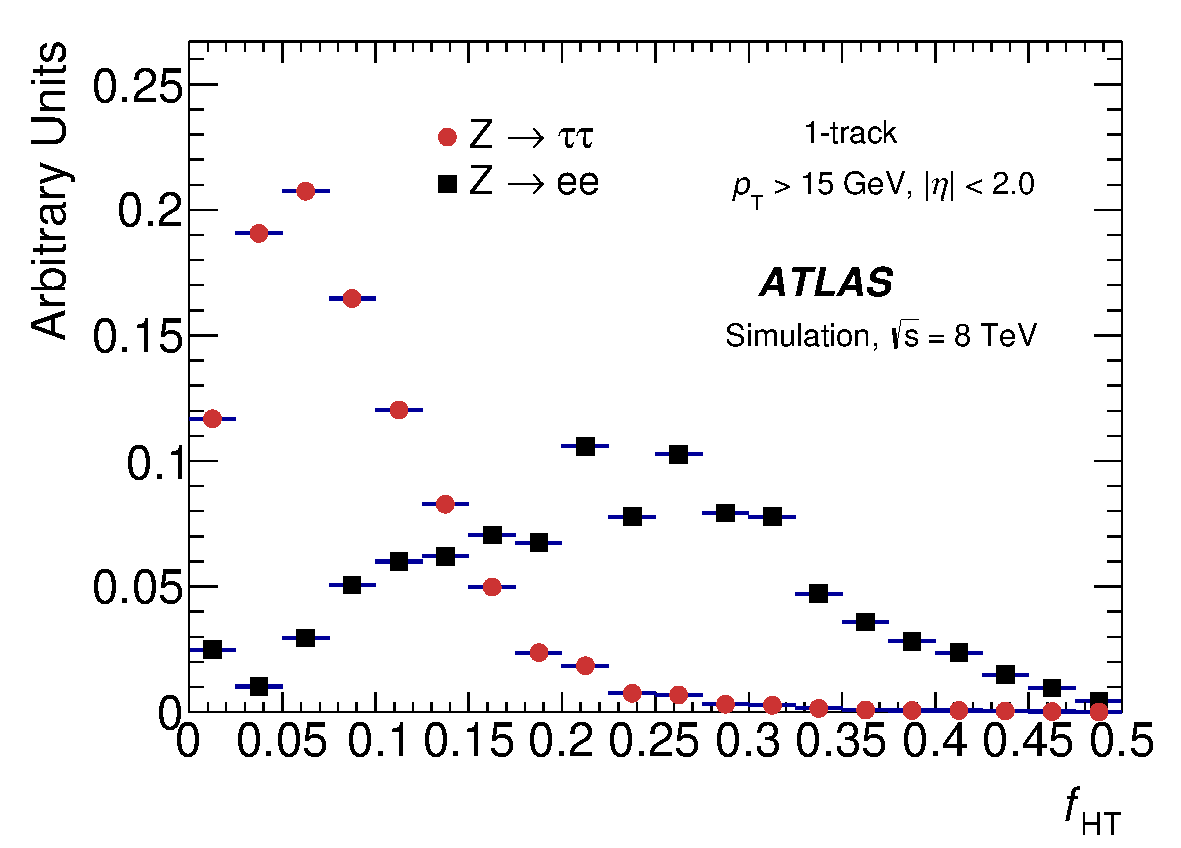
\includegraphics[width=0.48\textwidth]{figures/PERF-2013-06/fig_08a}
  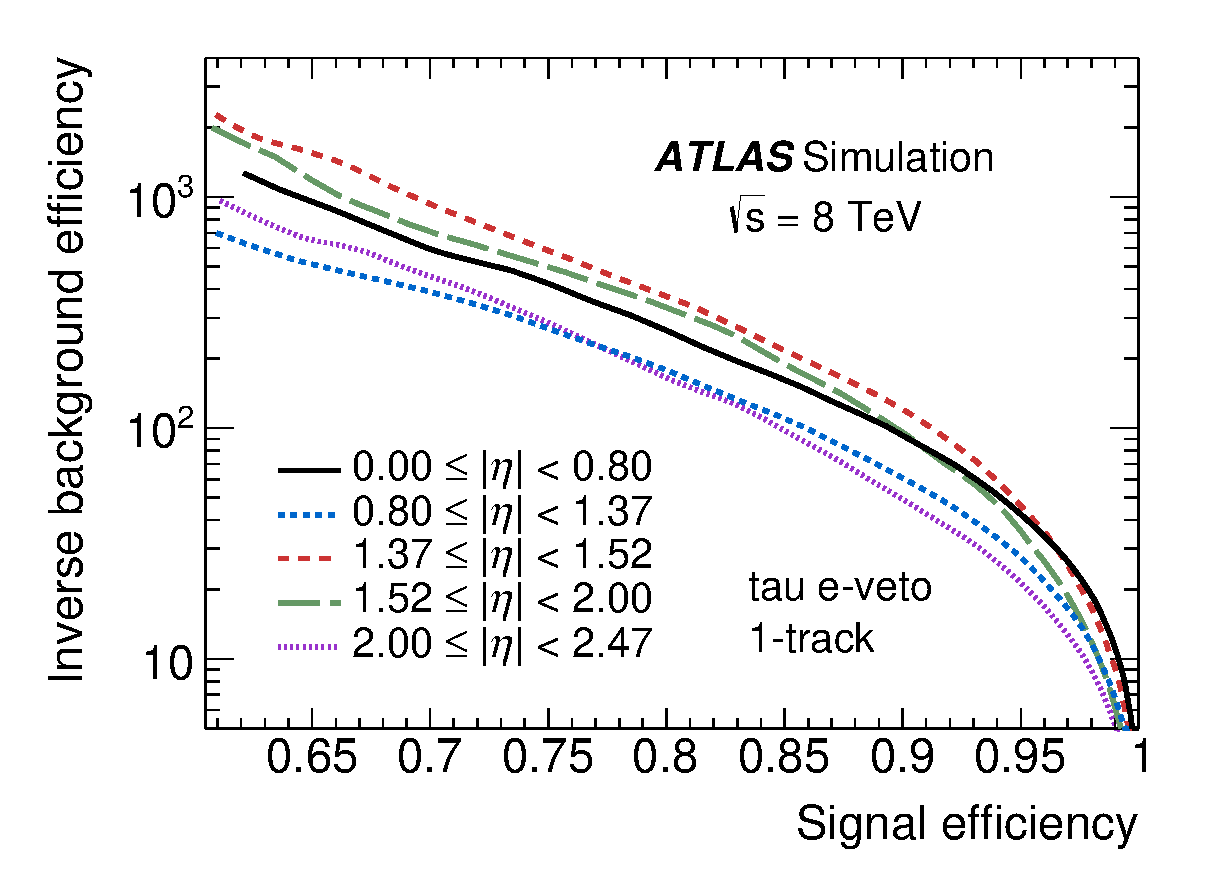
\includegraphics[width=0.48\textwidth]{figures/PERF-2013-06/fig_09}
  \caption{Variables.}
  \label{fig:taus-electronfakes1}
\end{figure}

\begin{figure}[tp]
  \centering
  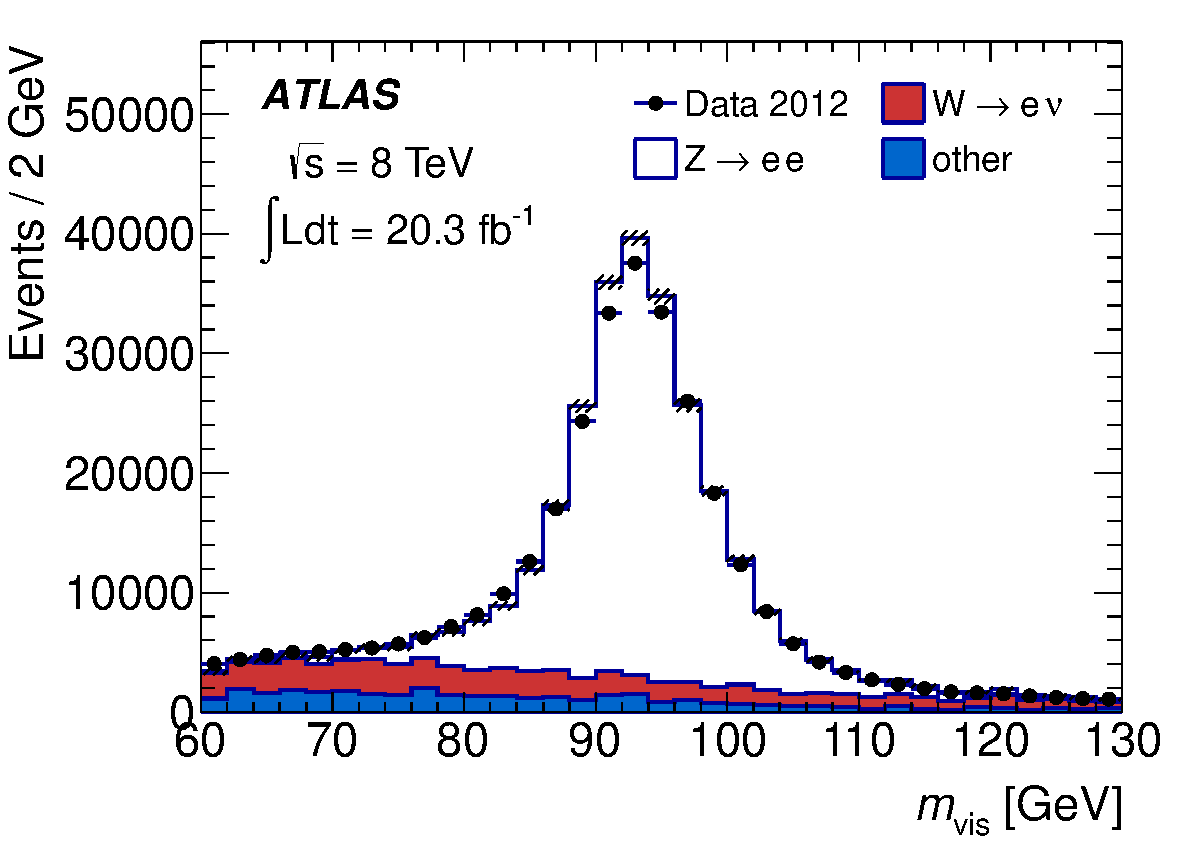
\includegraphics[width=0.48\textwidth]{figures/PERF-2013-06/fig_14a}
  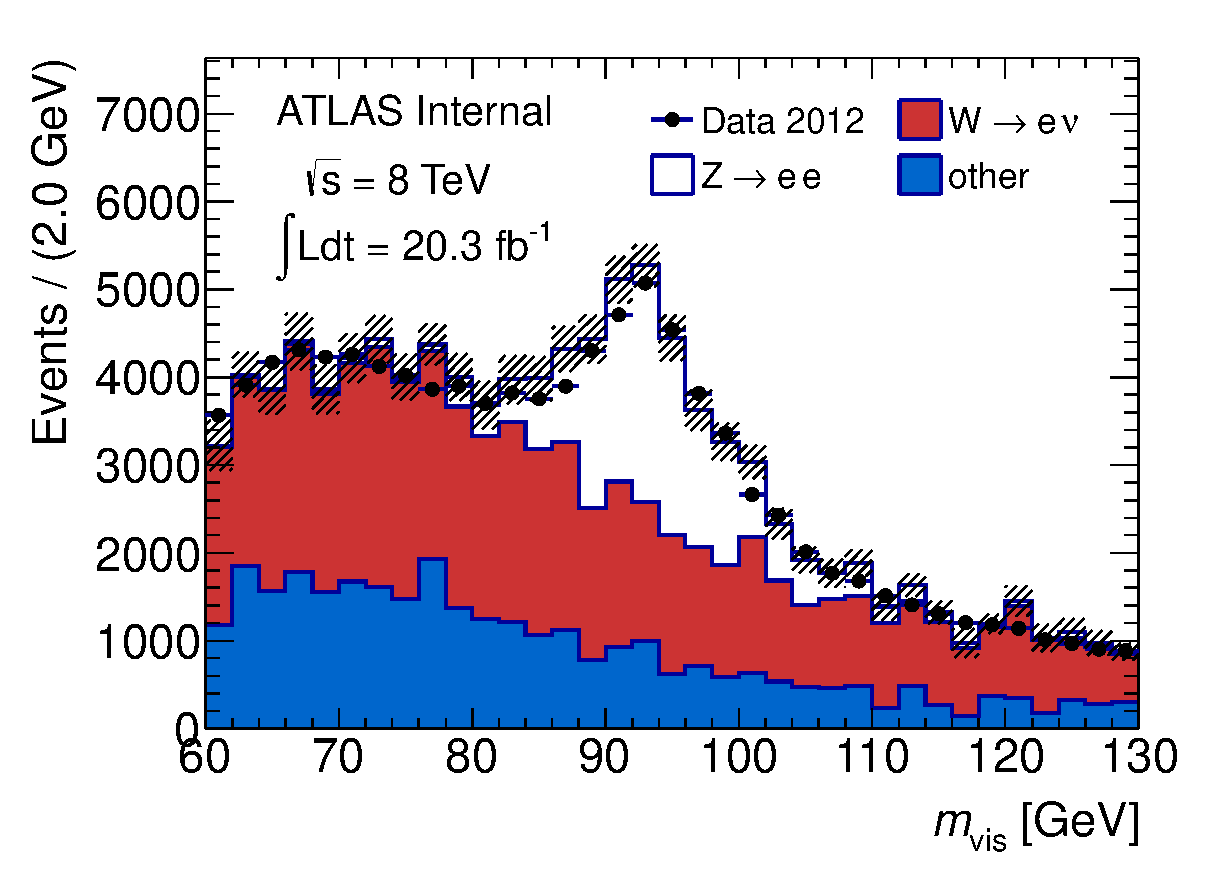
\includegraphics[width=0.48\textwidth]{figures/PERF-2013-06/eveto_mvis_mediumID_loosePPOLR_looseeveto}
  \caption{Variables.}
  \label{fig:taus-electronfakes2}
\end{figure}


